% Confounder structural DAG (Supplementary Figure 2), TikZ standalone.
% Body composition is a CONFOUNDER (fatlean -> dsc); fatlean in the MSAS (red).
% Build (fontspec + Inter -> xelatex; run TWICE):
%   xelatex confounder.tex
% Output: confounder.pdf -> outputs/figures/final/supp-fig-2-confounder-dag.pdf

\documentclass[border=10pt]{standalone}
\usepackage{fontspec}
% BoldFont declared so the legend's \textbf{Nodes:}/\textbf{Edges:} resolve --- plain
% "Inter" ships no bold shape here, so the bold face is named explicitly.
\setsansfont{Inter}[BoldFont={Inter 18pt SemiBold}]
\renewcommand{\familydefault}{\sfdefault}
\usepackage{tikz}
\usetikzlibrary{arrows.meta, positioning, fit, backgrounds, calc}

\definecolor{stageSetup}{HTML}{CFD8EA}
\definecolor{stageLang}{HTML}{CFDFCD}
\definecolor{stageAuth}{HTML}{E3C2BC}
\definecolor{stageOut}{HTML}{D9D9D9}
\definecolor{dark}{HTML}{1E293B}
\definecolor{slate}{HTML}{64748B}
\definecolor{linegreen}{HTML}{3F7E4E}
\definecolor{linered}{HTML}{A85D52}
\definecolor{lineamber}{HTML}{C77B30}

\tikzset{
  font=\sffamily\footnotesize,
  exposure/.style={rectangle, rounded corners=4pt, draw=slate!75, line width=0.7pt,
                   fill=stageLang, text=dark, align=center,
                   minimum width=1.8cm, minimum height=0.95cm},
  outcome/.style={rectangle, rounded corners=4pt, draw=slate!75, line width=0.7pt,
                  fill=stageSetup, text=dark, align=center,
                  minimum width=1.6cm, minimum height=0.95cm},
  msas/.style={rectangle, rounded corners=4pt, draw=linered, line width=0.9pt,
               fill=stageAuth, text=dark, align=center,
               minimum width=1.5cm, minimum height=0.95cm},
  obs/.style={rectangle, rounded corners=4pt, draw=slate!75, line width=0.7pt,
              fill=white, text=dark, align=center,
              minimum width=1.5cm, minimum height=0.85cm},
  latent/.style={rectangle, rounded corners=4pt, draw=slate!85, line width=0.7pt, dashed,
                 fill=stageOut, text=dark, align=center,
                 minimum width=1.7cm, minimum height=0.95cm},
  causal/.style={-{Latex[length=2.6mm]}, draw=linegreen, line width=1.4pt},
  conf/.style={-{Latex[length=2.6mm]}, draw=linered, line width=1.0pt},
  latentedge/.style={-{Latex[length=2.6mm]}, draw=lineamber, line width=1.0pt, dashed},
  other/.style={-{Latex[length=2.6mm]}, draw=slate, line width=0.6pt, opacity=0.85},
  anno/.style={font=\sffamily\itshape\small, text=slate},
  legend/.style={font=\sffamily\scriptsize, text=dark, align=center},
}

% ---- legend helpers ----
% The swatch macros take a style/colour name, so they resolve against THIS file's own
% \tikzset above -- the legend therefore cannot drift from what is drawn. The legend
% sits below the caption, so the standalone bounding box grows downward only.
% Vertical centring is set PER SWATCH TYPE, and each value was swept INSIDE this
% figure and measured at 1200 dpi against its own adjacent label. A single shared
% knob does not work here: the three macros build different objects (a tikz node, a
% plain rule, a tikz path) and they do not land alike for a given offset in this
% file's context. If they need retuning, sweep them in the figure itself: a reduced
% test case lacks the global font= in \tikzset that the nested \tikz swatches inherit,
% and will centre them correctly there while leaving them ~3 pt low here.
\newcommand{\swnode}{-1.5ex}                       % \lnode  (tikz node)
\newcommand{\swdash}{-0.65ex}                      % \ledgedash (tikz path)
\newcommand{\swrule}{\dimexpr0.5ex-0.55pt\relax}   % \ledge (rule lift, from its bottom)
\newcommand{\lnode}[1]{\tikz[baseline=\swnode]\node[#1, minimum width=0.38cm, minimum height=0.24cm, inner sep=1.5pt]{};}
\newcommand{\ledge}[1]{{\color{#1}\rule[\swrule]{0.5cm}{1.1pt}}}
\newcommand{\ledgedash}[1]{\tikz[baseline=\swdash]\draw[#1, line width=1.1pt, dashed](0,0)--(0.5cm,0);}
% Entry wrappers: \mbox keeps a swatch glued to its label so the line can only break
% BETWEEN entries, never inside one (otherwise it hyphenates to "confound-/ing path").
\newcommand{\lentry}[2]{\mbox{\lnode{#1}\ #2}}
\newcommand{\eentry}[2]{\mbox{\ledge{#1}\ #2}}
\newcommand{\eentrydash}[2]{\mbox{\ledgedash{#1}\ #2}}

\begin{document}
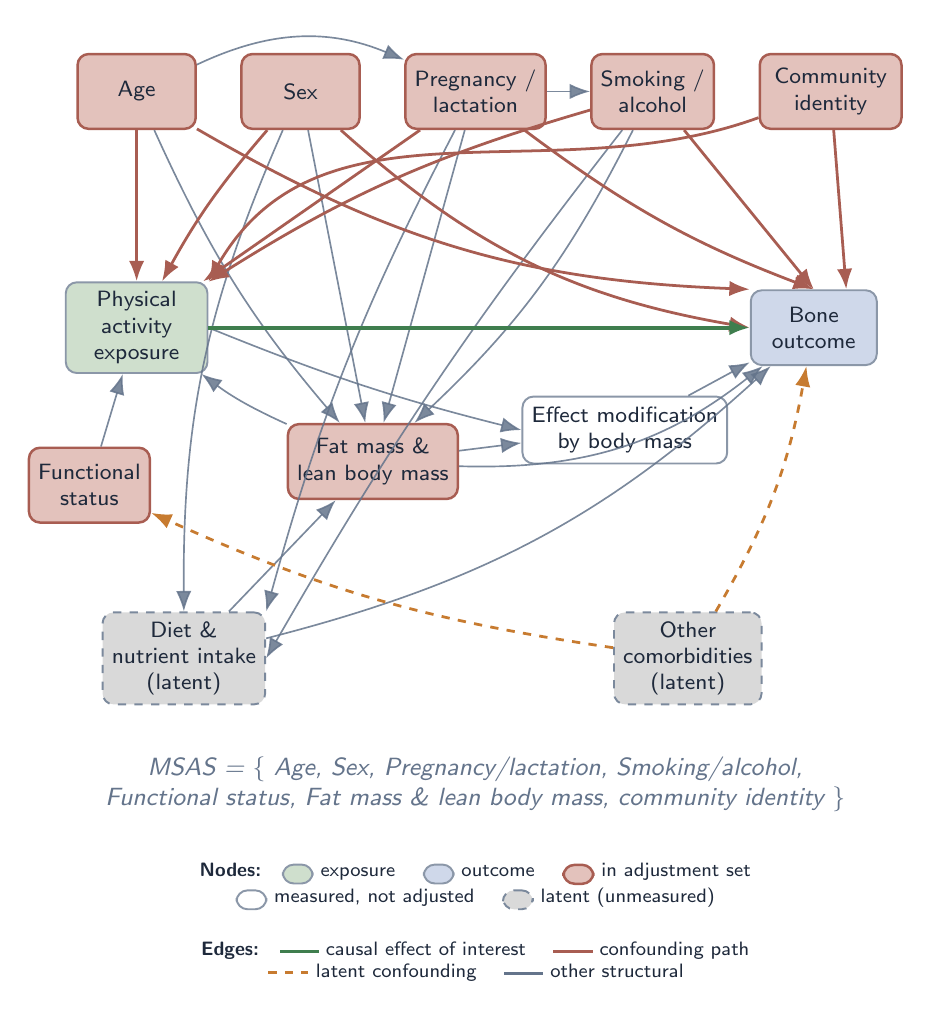
\begin{tikzpicture}

% #1 = x-offset (0 here), #2 = fatlean style (msas), #3 = body-comp edge key (conf)
\newcommand{\drawpanel}[3]{%
  \begin{scope}[xshift=#1 cm]
    \node[msas]     (age)  at (0.0, 6.2) {Age};
    \node[msas, right=0.55cm of age] (sex)  {Sex};
    \node[msas, right=0.55cm of sex] (pl)   {Pregnancy /\\ lactation};
    \node[msas, right=0.55cm of pl]  (smk)  {Smoking /\\ alcohol};
    \node[msas, minimum width=1.8cm, right=0.55cm of smk] (vill) {Community\\ identity};

    \node[exposure] (dsc)  at (0.0, 3.2) {Physical\\ activity\\ exposure};
    \node[outcome]  (osteo) at (8.6, 3.2) {Bone\\ outcome};
    \node[obs]      (em)   at (6.2, 1.9) {Effect modification\\ by body mass};
    \node[#2]       (fl)   at (3.0, 1.5) {Fat mass \&\\ lean body mass};

    \node[msas]     (fs)   at (-0.6, 1.2) {Functional\\ status};
    \node[latent]   (diet) at (0.6, -1.0) {Diet \&\\ nutrient intake\\ (latent)};
    \node[latent]   (comorb) at (7.0, -1.0) {Other\\ comorbidities\\ (latent)};

    % --- grey "other" edges ---
    \draw[other] (age) to[bend left=24] (pl);
    \draw[other] (pl)  -- (smk);
    \draw[other] (age) to[bend right=8] (fl);
    \draw[other] (sex) -- (fl);
    \draw[other] (pl)  -- (fl);
    \draw[other] (smk) to[bend left=10] (fl);
    \draw[other] (sex) to[bend right=12] (diet.north);
    \draw[other] (pl)  to[bend right=6]  (diet.north east);
    \draw[other] (smk) to[bend right=4]  (diet.east);
    \draw[other] (dsc.east) to[bend right=4] (em.west);
    \draw[other] (fl)  to[bend right=20] (osteo);
    \draw[other] (fl)  -- (em);
    \draw[other] (em)  -- (osteo);
    \draw[other] (diet) to[bend right=14] (osteo);
    \draw[other] (diet) -- (fl);
    \draw[other] (fs)  -- (dsc);
    \ifnum\pdfstrcmp{#3}{med}=0
      \draw[other] (dsc) to[bend right=6] (fl);
    \else
      \draw[other] (fl) to[bend left=6]  (dsc);
    \fi

    % --- red confounder edges: {age,sex,pl,smk,vill} -> {dsc,osteo} ---
    \draw[conf] (age) -- (dsc);
    \draw[conf] (age) to[bend right=14] (osteo.north west);
    \draw[conf] (sex) to[bend right=6] (dsc);
    \draw[conf] (sex) to[bend right=16] (osteo.west);
    \draw[conf] (pl)  -- (dsc);
    \draw[conf] (pl)  to[bend right=8] (osteo.north);
    \draw[conf] (smk) to[bend right=8] (dsc);
    \draw[conf] (smk) -- (osteo.north);
    \draw[conf] (vill) to[out=200,in=60] (dsc.north east);
    \draw[conf] (vill) -- ([xshift=-4mm]osteo.north east);

    % --- amber dashed latent edges ---
    \draw[latentedge] (comorb) to[bend left=8]  (fs);
    \draw[latentedge] (comorb) to[bend right=10] (osteo);

    % --- green causal edge (drawn last) ---
    \draw[causal] (dsc) -- (osteo);
  \end{scope}
}

\drawpanel{0}{msas}{conf}

\node[anno, align=center] (msascap) at (4.3, -2.6)
  {MSAS = \{ Age, Sex, Pregnancy/lactation, Smoking/alcohol,\\ Functional status, Fat mass \& lean body mass, community identity \}};

% --- legend (adaptive: only the roles and edge classes this DAG actually uses) ---
% Note vs. the mediator DAG: fat mass & lean body mass is drawn msas/red here, because
% under the confounder structure it is upstream of activity and IS adjusted for.
\node[legend, text width=10.6cm, below=4mm of msascap] (legnodes) {%
  \textbf{Nodes:}\ \, \lentry{exposure}{exposure} \quad
  \lentry{outcome}{outcome} \quad
  \lentry{msas}{in adjustment set} \quad
  \lentry{obs}{measured, not adjusted} \quad
  \lentry{latent}{latent (unmeasured)}};
\node[legend, text width=10.6cm, below=1.6mm of legnodes] {%
  \textbf{Edges:}\ \, \eentry{linegreen}{causal effect of interest} \quad
  \eentry{linered}{confounding path} \quad
  \eentrydash{lineamber}{latent confounding} \quad
  \eentry{slate}{other structural}};

\end{tikzpicture}
\end{document}
